\documentclass{article}
\usepackage{enumitem}
\usepackage{listings}
\usepackage{amsfonts}
\usepackage{latexsym}
\usepackage{fullpage}
\usepackage{graphicx}
\usepackage{paralist}
\usepackage{tikz-timing}

\lstdefinelanguage{VHDL}{
  morekeywords={
    library,use,all,ENTITY,IS,PORT,IN,OUT,end,architecture,of,
    begin,and, ARCHITECTURE, IF, THEN, SIGNAL,END, PROCESS
  },
  morecomment=[l]--
}

\usepackage{xcolor}
\colorlet{keyword}{blue!100!black!80}
\colorlet{comment}{green!90!black!90}
\lstdefinestyle{vhdl}{
  language     = VHDL,
  basicstyle   = \ttfamily\scriptsize,
  keywordstyle = \color{keyword}\bfseries\ttfamily,
  commentstyle = \color{comment}\ttfamily,	
  tabsize=1
}

\renewcommand{\lstlistingname}{Code}

% Default margins are too wide all the way around. I reset them here
\setlength{\topmargin}{-.5in}
\setlength{\textheight}{9in}
\setlength{\oddsidemargin}{.125in}
\setlength{\textwidth}{6.25in}


%\let\oldenumerate\enumerate
%\renewcommand{\enumerate}{
  %\oldenumerate
  %\setlength{\itemsep}{1pt}
  %\setlength{\parskip}{0pt}
  %\setlength{\parsep}{0pt}
%}


\begin{document}
\title{EECS112L Organization of Digital Computers Lab}
\author{\textbf{Lab 2} \textbf{Single-cycle ARM Datapath and Control - Complete} \\ \\
Group name: Three Musketeers \\ \\ Group ID: 118 \\ \\ Student name: \\ Raymond Wang \\ Jared Lim\\ Heyang Chen \\ \\ Student ID: \\17769107~\\31633414~\\55554499~\\ \\ 
EECS Department\\ Henry Samueli School of Engineering \\ University of California, Irvine \\ \\
{February, 28, 2017}} 


\date{}
\maketitle

\newpage

\section{Description of this Lab}

In this lab, We started from the basis of last lab and adding more features including data processing instructions, branch and link, and byte-size store/load instruction.

\section{Block Diagram}

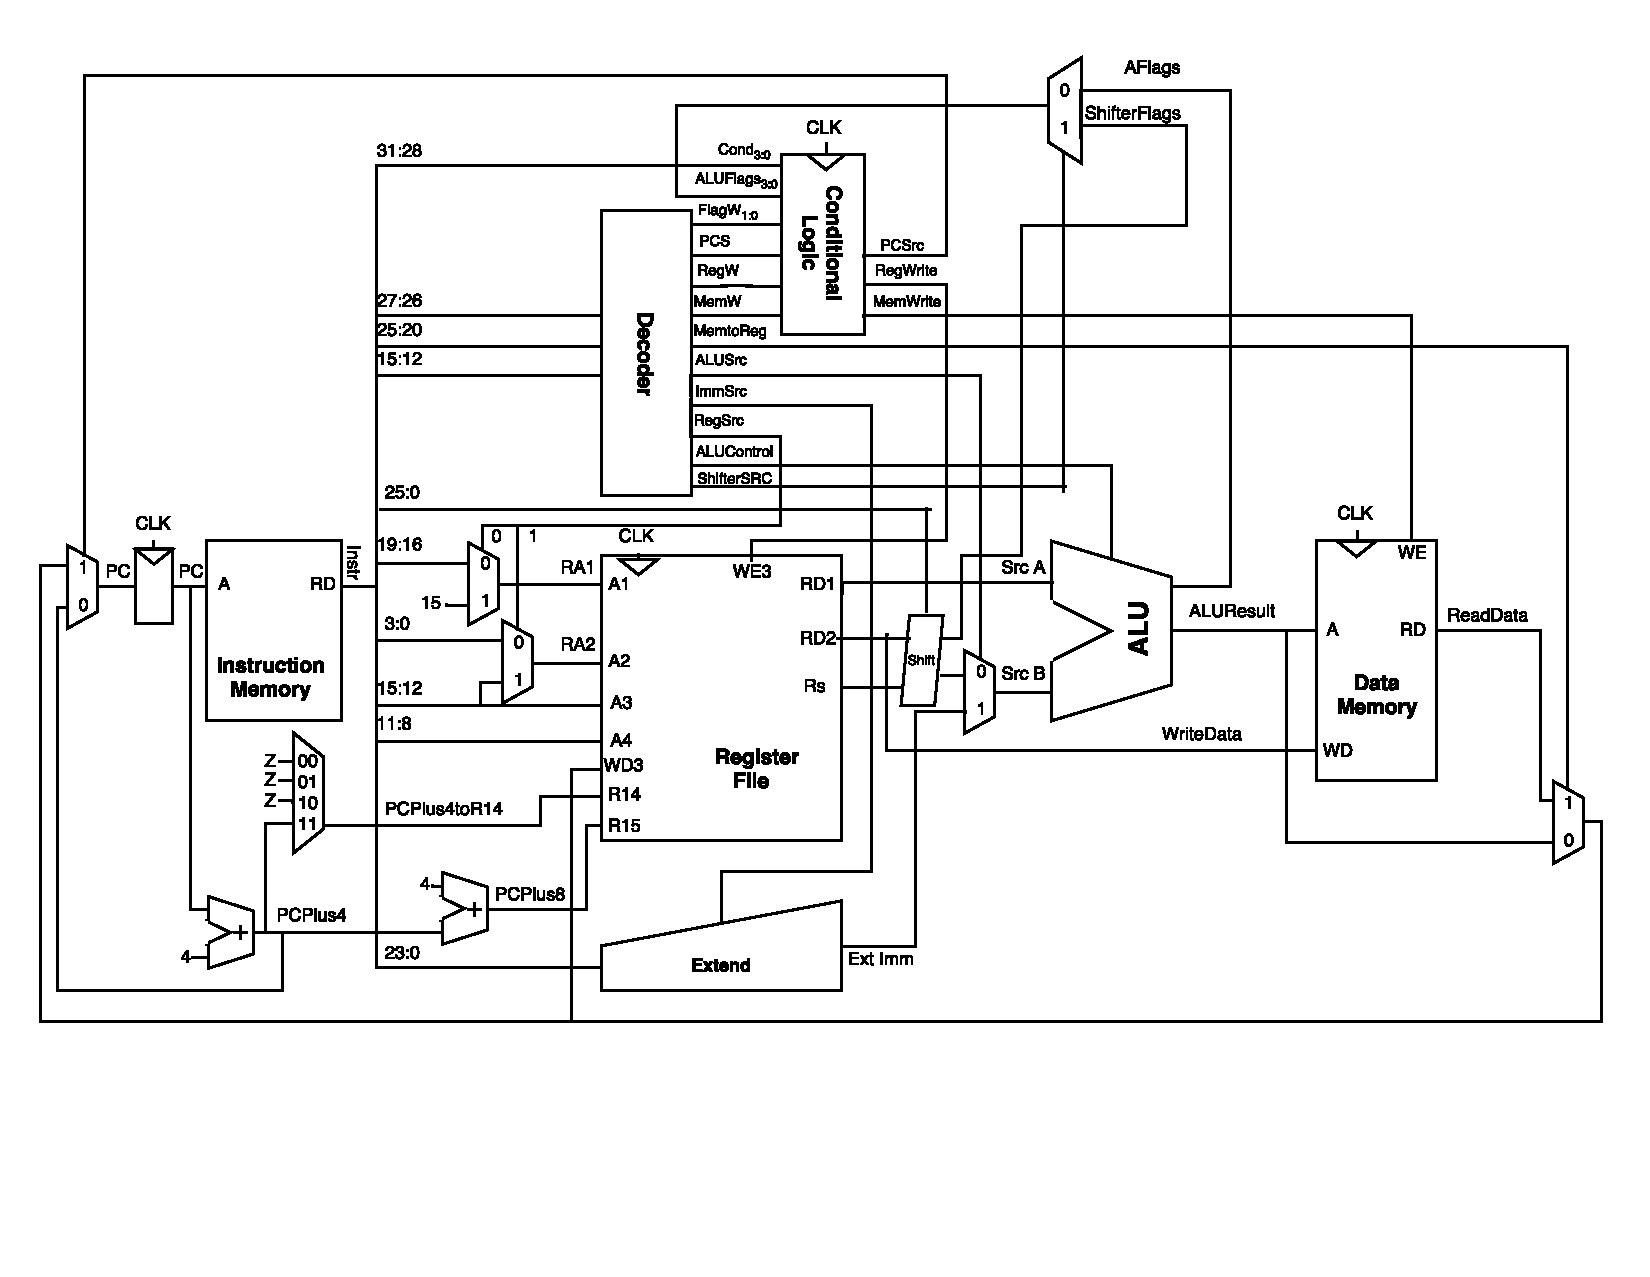
\includegraphics[width=1.0\textwidth]{SingleCycleProcessor.pdf}

\section{Design Architecture}

In designing this lab, we followed ideas mainly from supplement reference book and ARM manual provided by TA. First of all, we designed branch and link. As shown in the block diagram, we designed a new module of 4-way multiplexer and have PCPlus4 input this 4-way multiplexer and then goes into Register 14 on register file. 
\newline
Then for the immediate-shifted and register-shifted register instruction. We actually create a new shift register, get the shift done there and then push to multiplexer before ALU. In this way, it won't make ALU become confusing and having a whole lot of new input/output in ALU. We first having Instr[11:8] input into regfile as Ra4 and get the Rs by given Rs = R15[Ra4] which is the register shift amount. Then Instr[25] comes into shift as I bit deciding whether it is Mov or the rest shift operation. Then Instr[4] decide whether it is a immediate shift or register shift. Since we have shift done before going into ALU, we also have shifter output ShifterFlags similar to ALUFlags. Then adding a ShifterSrc to decoder in order to decide in the multiplexer on which flags we are using to input into condlogic as ALUFlags.
\newline
For ALU, we have changed based on the design of last time and making operation code from 2 bits to 4 bits in order to support all the data-processing instructions. All of the design follows the table given in lab description.
\newline
For store byte, store half, load byte and load half, we made changes in decoder as well as controller. We added a 4 bit Byte-enable(be) and output that with different value according to different situation generating by operation code, operation code2, Funct[5] and Funct[2].

\section{Simulation Waveform}


\section{Examine the Correctness}



\end{document}
